\documentclass[compress]{beamer}
\usepackage{ifthen,verbatim}

\newcommand{\isnote}{}
\xdefinecolor{lightyellow}{rgb}{1.,1.,0.25}
\xdefinecolor{darkblue}{rgb}{0.1,0.1,0.7}

%% Uncomment this to get annotations
%% \def\notes{\addtocounter{page}{-1}
%%            \renewcommand{\isnote}{*}
%% 	   \beamertemplateshadingbackground{lightyellow}{white}
%%            \begin{frame}
%%            \frametitle{Notes for the previous page (page \insertpagenumber)}
%%            \itemize}
%% \def\endnotes{\enditemize
%% 	      \end{frame}
%%               \beamertemplateshadingbackground{white}{white}
%%               \renewcommand{\isnote}{}}

%% Uncomment this to not get annotations
\def\notes{\comment}
\def\endnotes{\endcomment}

\setbeamertemplate{navigation symbols}{}
\setbeamertemplate{headline}{\mbox{ } \hfill
\begin{minipage}{5.5 cm}
\vspace{-0.75 cm} \small
\end{minipage} \hfill
\begin{minipage}{4.5 cm}
\vspace{-0.75 cm} \small
\begin{flushright}
\ifthenelse{\equal{\insertpagenumber}{1}}{}{Jim Pivarski \hspace{0.2 cm} \insertpagenumber\isnote/\pageref{numpages}}
\end{flushright}
\end{minipage}\mbox{\hspace{0.2 cm}}\includegraphics[height=1 cm]{../cmslogo} \hspace{0.1 cm} \includegraphics[height=1 cm]{../tamulogo} \hspace{0.01 cm} \vspace{-1.05 cm}}

\begin{document}

\scriptsize

\begin{frame}
\frametitle{Tracker/muon relative $z$ position measurement}
\begin{itemize}\setlength{\itemsep}{0.1 cm}
\item Every globalMuon track measures tracker/muon displacement, but
  low-momentum tracks are dominated by multiple scattering (tails)

\vspace{0.05 cm}
\begin{itemize}\scriptsize\setlength{\itemsep}{0.1 cm}
\item want to take a mean of the highest-momentum tracks
\item plot alignment correction versus curvature ($q/p_T$)
\item Taylor expansion around point of infinite momentum ($q/p_T = 0$)
\item quadratic fit: $p_0$ is misalignment (independent of tracks), $p_1$ is $\vec{B}$ error (antisymmetric with $q$), $p_2$ is multiple \mbox{scattering (symmetric with $q$)\hspace{-1 cm}}
\end{itemize}

\item Moved tracker to $z = -3.8$~mm in GlobalPositionRcd (from two iterations):

\textcolor{darkblue}{\tiny \tt /afs/cern.ch/cms/CAF/CMSALCA/ALCA\_MUONALIGN/SWAlignment/CRAFTwheeldisk/CRAFT\_GlobalPositionRcd.db}
\end{itemize}

\vspace{0.1 cm}
\begin{columns}
\column{0.3\linewidth}
Histogram of track-by-track $z$ residuals

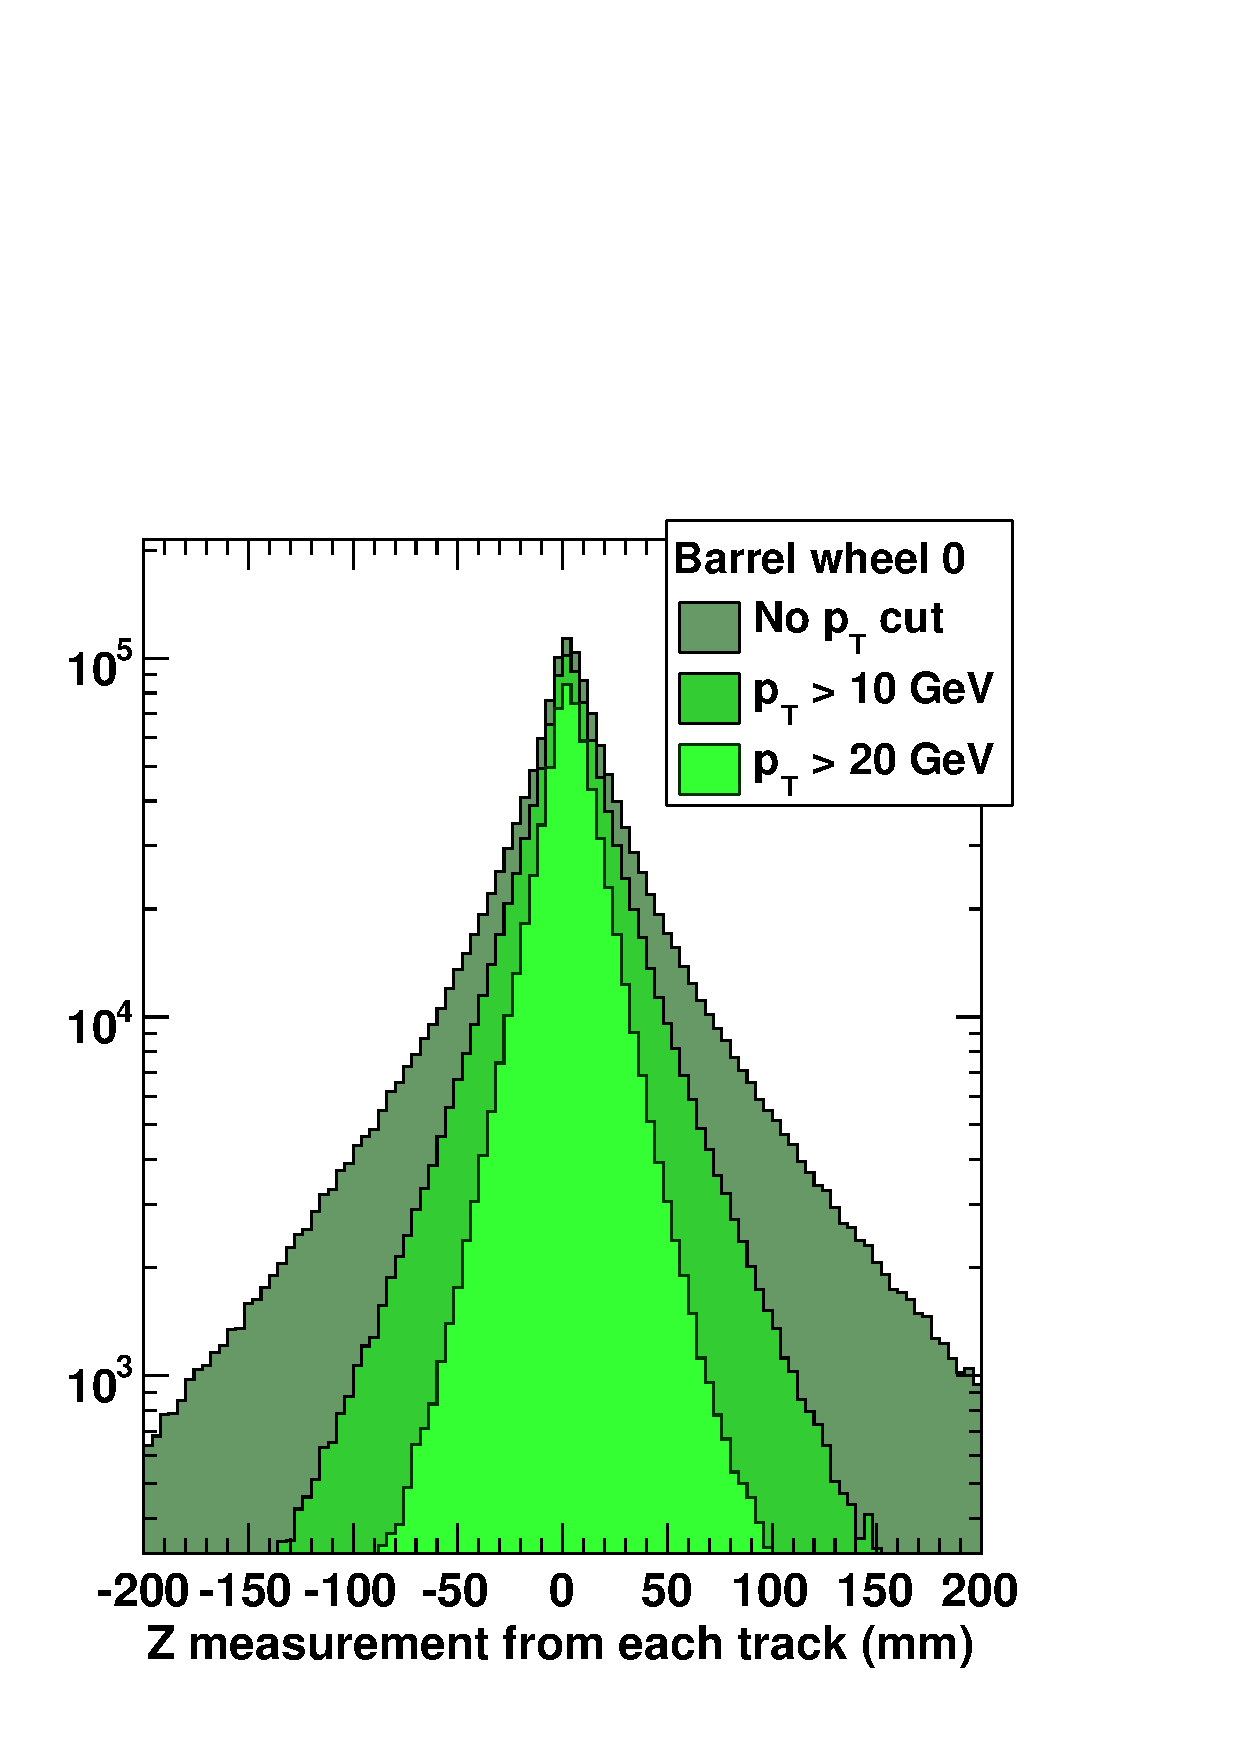
\includegraphics[width=\linewidth]{Zparameter_wh0.pdf}
\column{0.35\linewidth}
\mbox{ } \hfill Profile of iteration 0 \hfill \mbox{ }

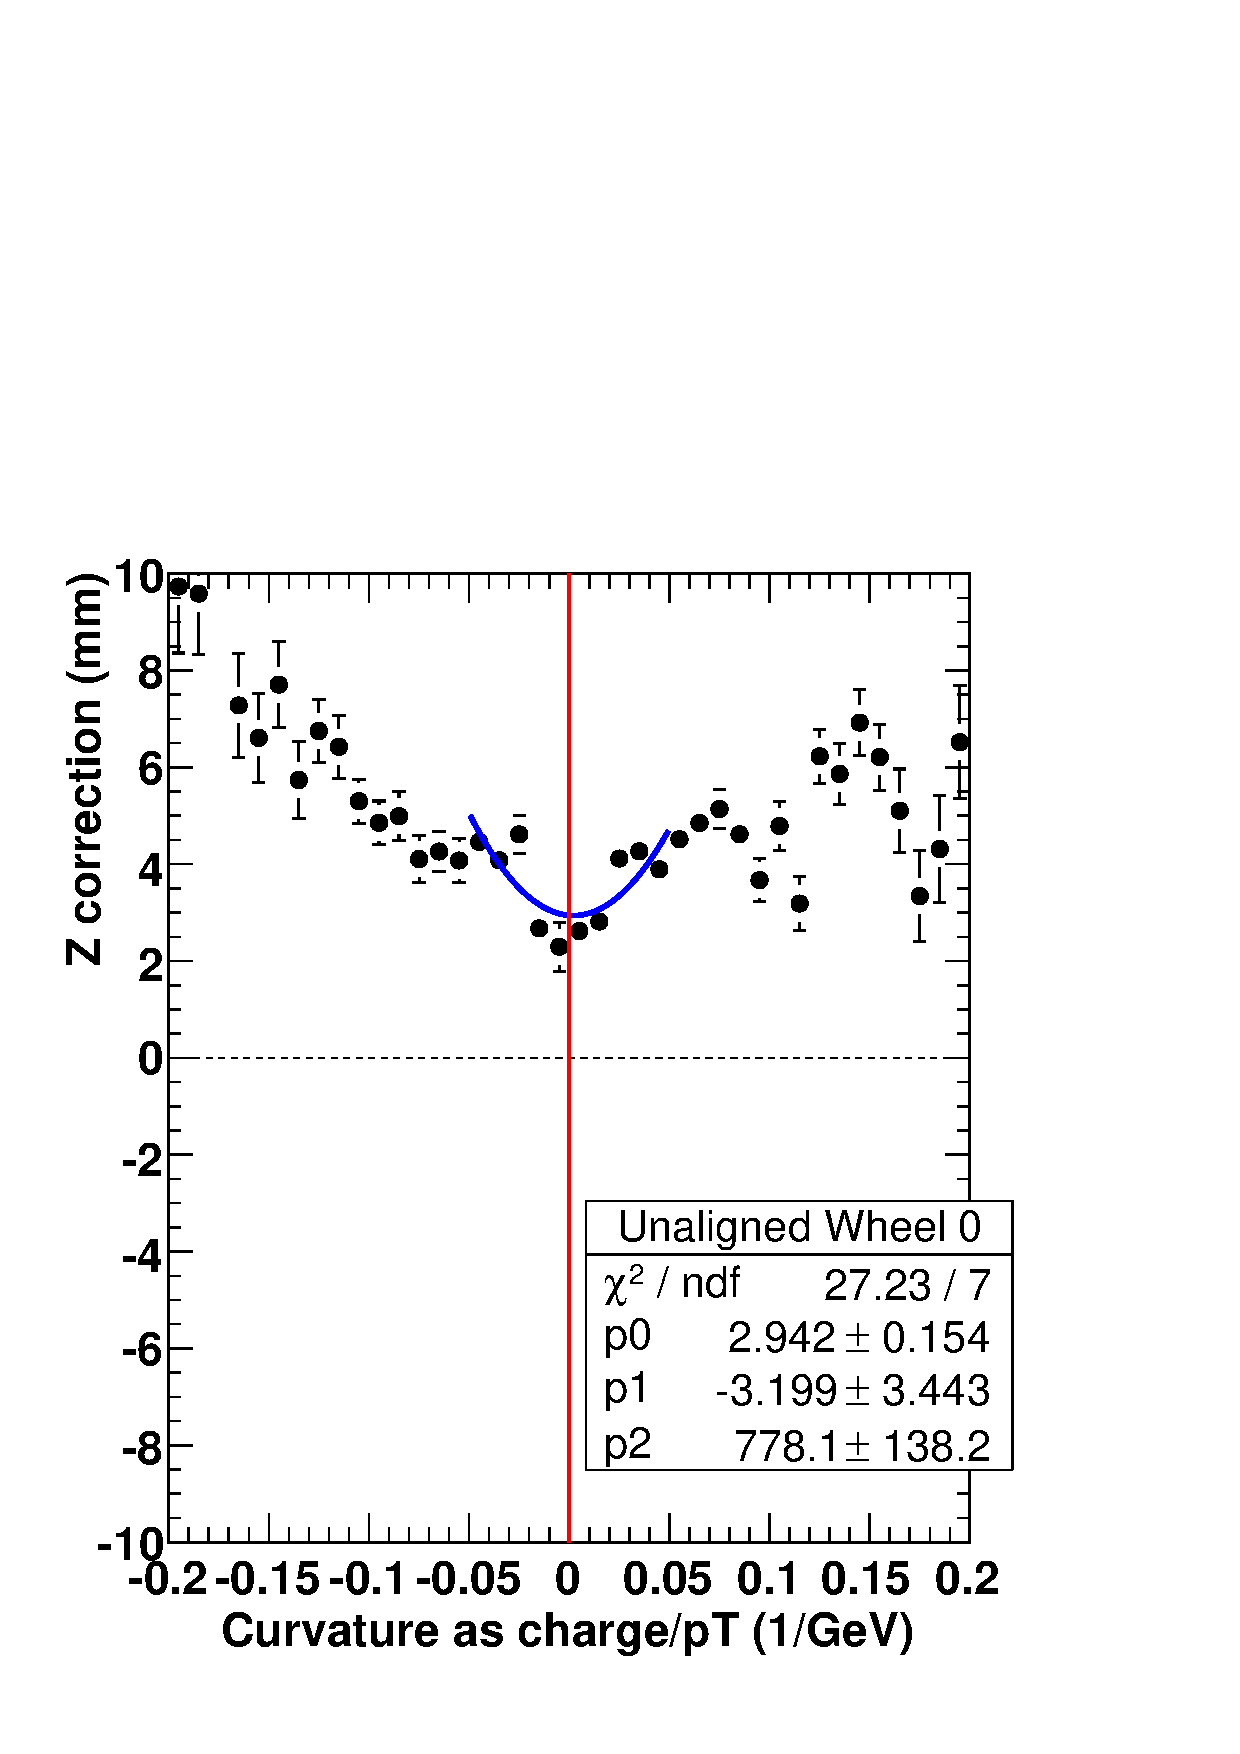
\includegraphics[width=\linewidth]{ZvsCurvature_wh0_unaligned.pdf}
\column{0.35\linewidth}
\mbox{ } \hfill Profile of iteration 2 \hfill \mbox{ }

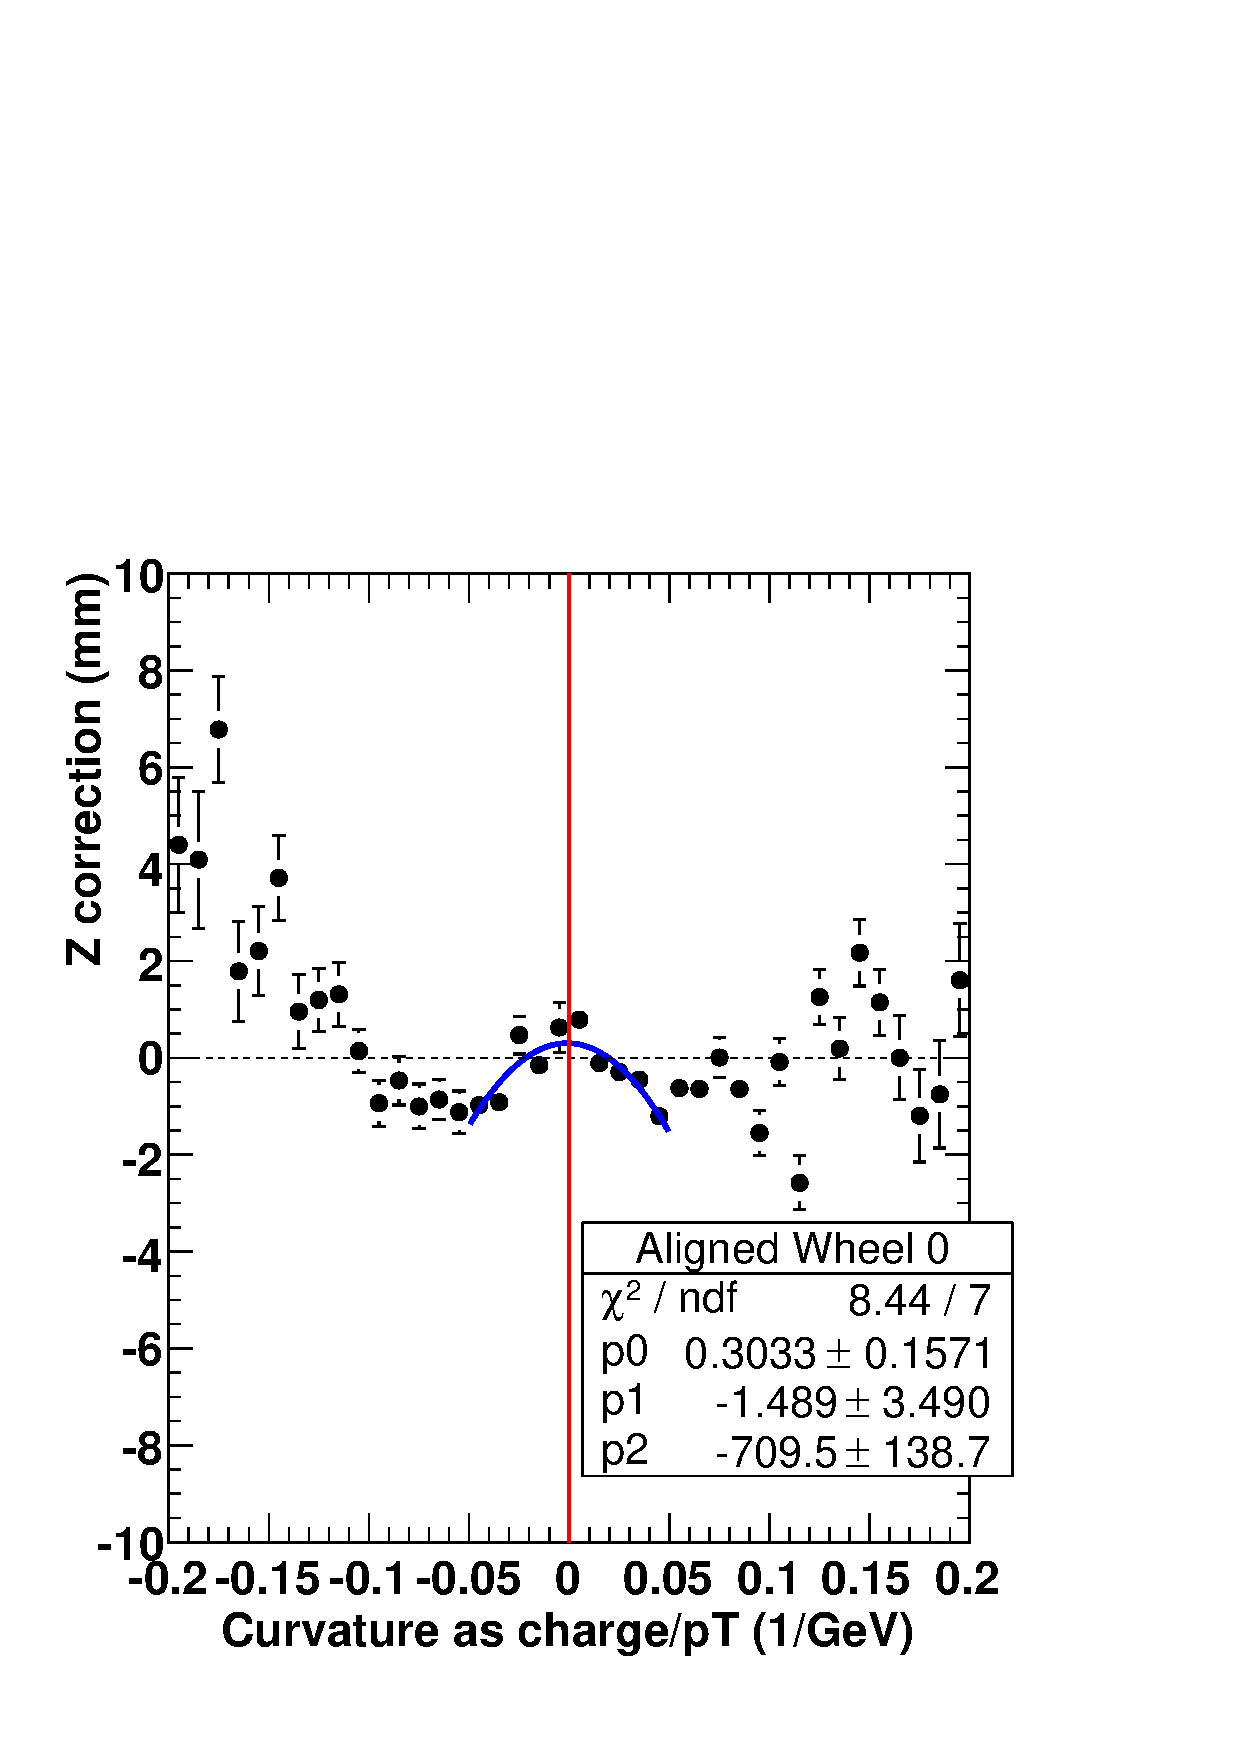
\includegraphics[width=\linewidth]{ZvsCurvature_wh0_aligned.pdf}
\end{columns}
\label{numpages}
\end{frame}

%% \begin{columns}
%% \column{0.5\linewidth}
%% \hfill 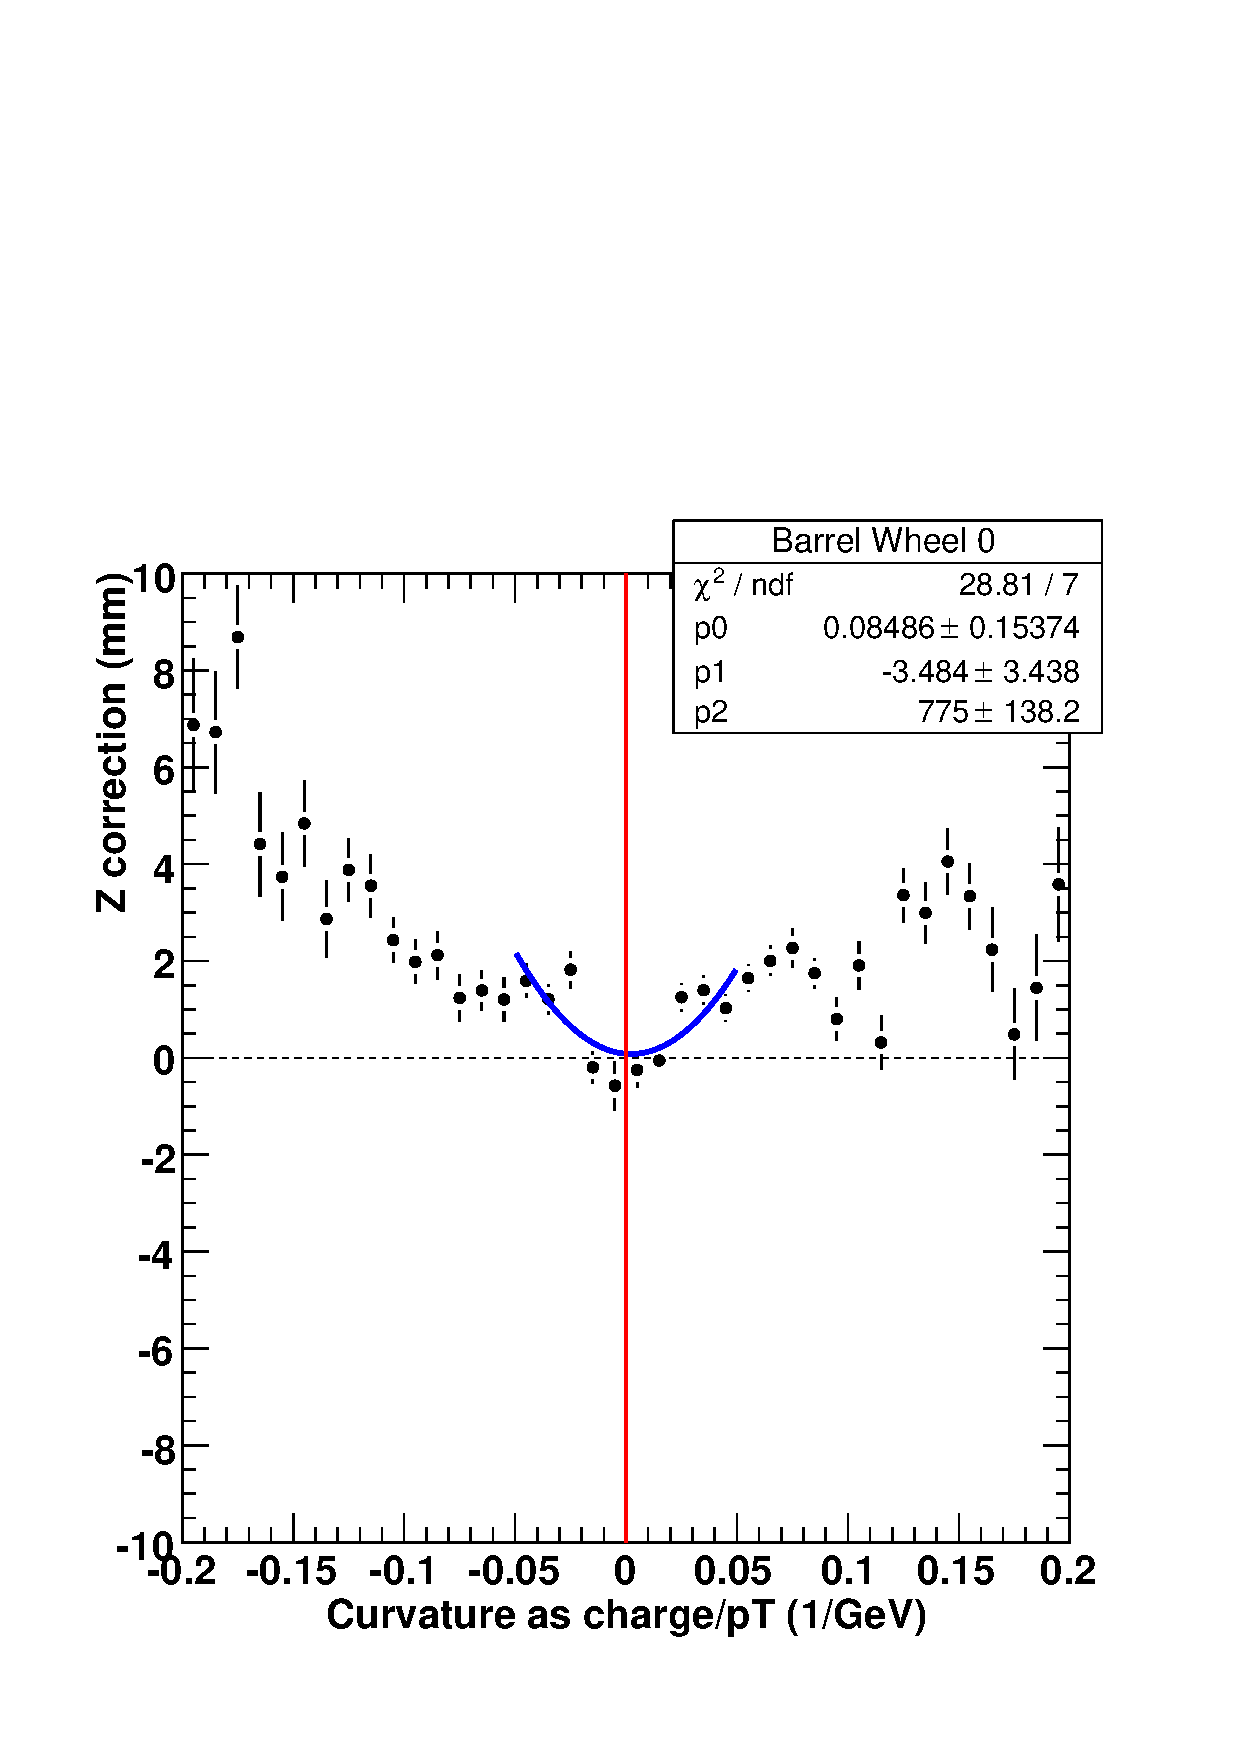
\includegraphics[width=0.8\linewidth]{ZvsCurvature_wh0_translateonly.pdf}

%% \column{0.5\linewidth}
%% 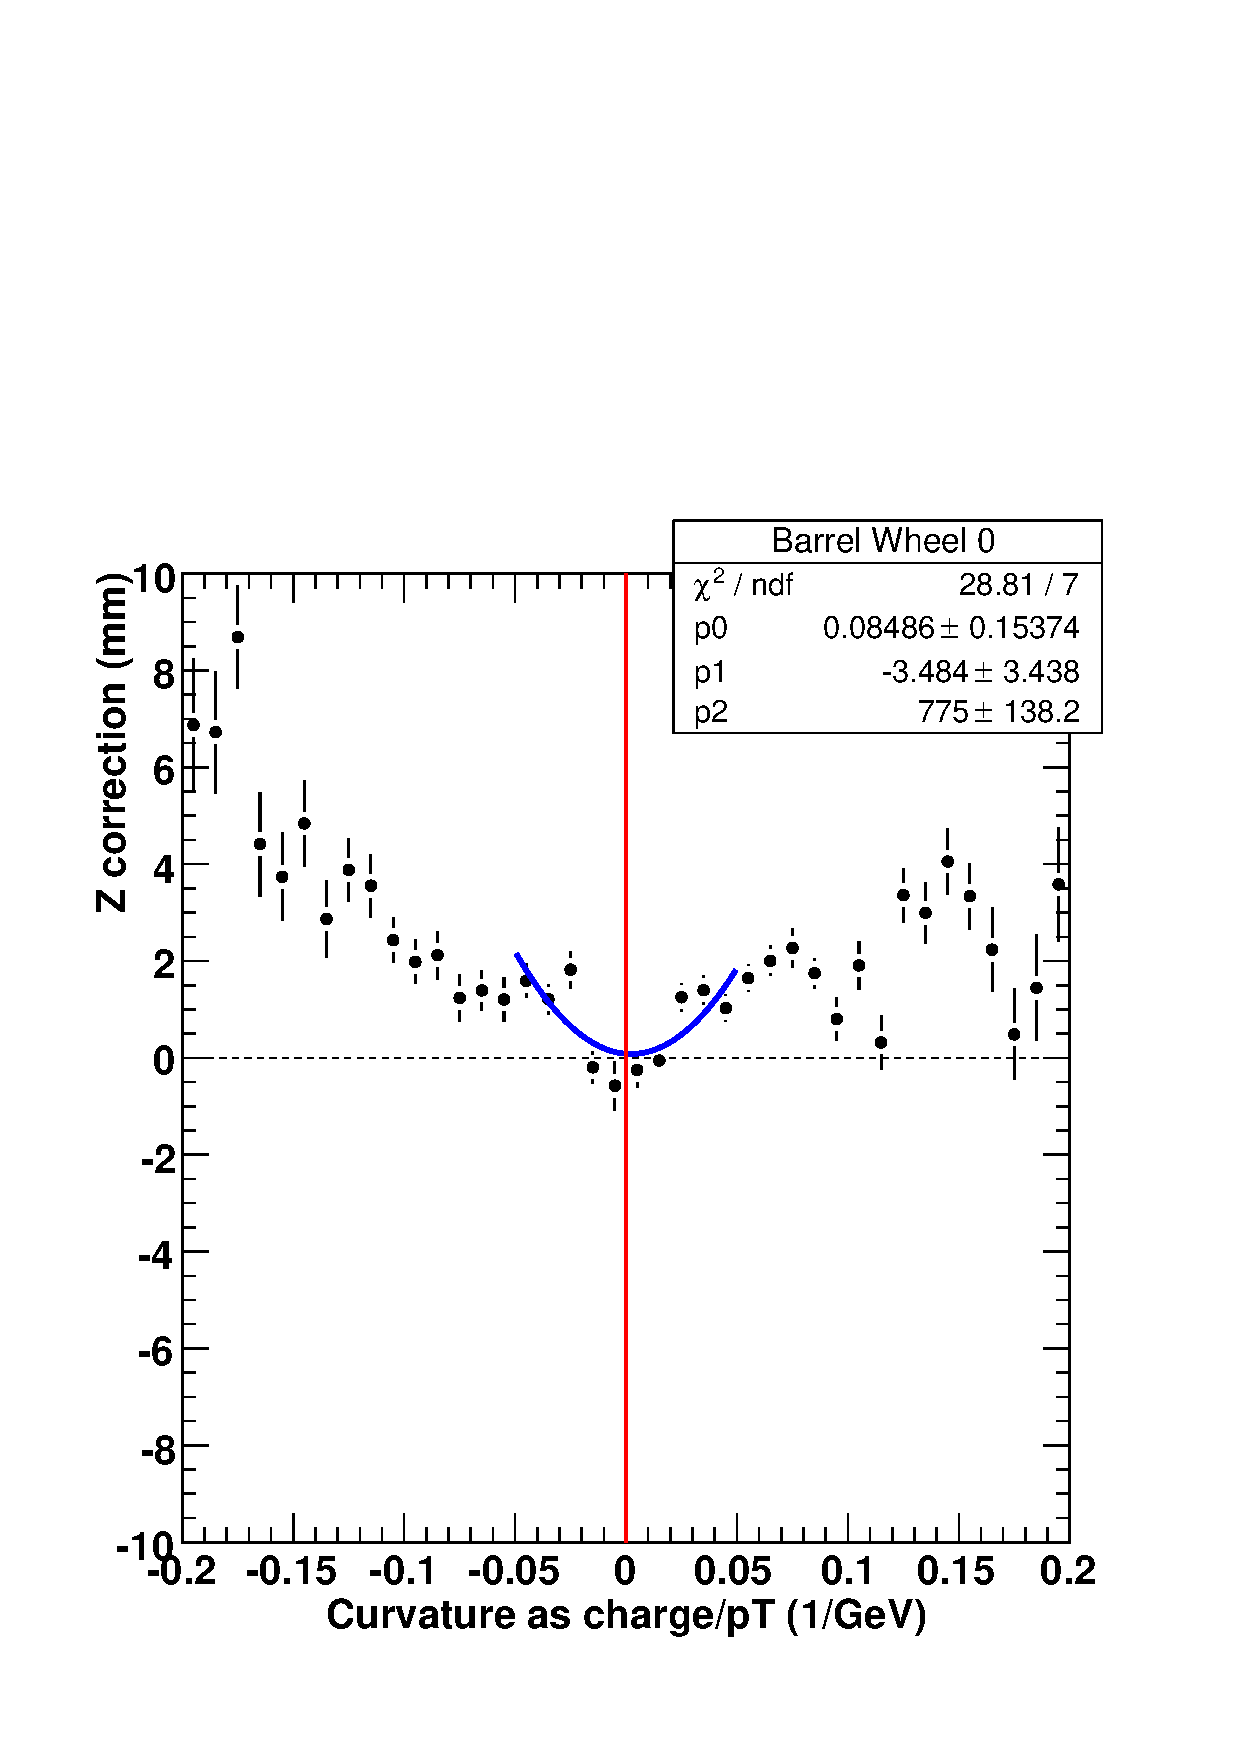
\includegraphics[width=0.8\linewidth]{ZvsCurvature_wh0_translateonly.pdf}
%% \end{columns}




%% \begin{frame}
%% \frametitle{Status of track-based procedures}
%% \begin{itemize}\setlength{\itemsep}{0.2 cm}
%% \item HIP and MillePede can produce alignments of the wheels and disks relative to the tracker with globalMuons
%% \item Constants are stable run-by-run
%% \item But they disagree with hardware constraints
%% \begin{itemize}
%% \item 2.5~mrad twist in $\phi_z$ from ME$-$2 to Wheel~0 disagrees with $\pm$0.5~mrad photogrammetry measurement
%% \item $z$ positions may or may not agree with optical measurements
%% \end{itemize}
%% \item $\chi^2$-invariant global distortions of the tracker {\it might} account for the difference
%% \item {\it If so,} track-based alignment would reverse its role and communicate physical measurements to the tracker
%% \end{itemize}
%% \end{frame}

%% \begin{frame}
%% \frametitle{Status of constants}
%% \begin{itemize}\setlength{\itemsep}{0.2 cm}
%% \item Track-based alignment moves wheels and disks as rigid bodies, so
%%   internal distortions must be supplied as input
%% \begin{itemize}\setlength{\itemsep}{0.1 cm}
%% \item Pre-CRAFT alignment of DT chambers within wheels available in CRAFT\_V3P (but updated yesterday?)
%% \item ME2,3,4 disk-curvatures from lasers were well studied but not in a
%%   CMSSW geometry record; I ported it as a public service
%% \item I received no concrete information about ME1; had to guess
%% \end{itemize}

%% \item Produced two sets of constants:
%% \begin{enumerate}\setlength{\itemsep}{0.1 cm}
%% \item Curved disks from lasers, centered whole muon system in $z$ with track-based alignment of wheel~0 \textcolor{darkblue}{(recommended)}
%% \begin{itemize}
%% \item Minimal use of track-based alignment
%% \item Global translation is not a bias but a coordinate definition
%% \end{itemize}
%% \item Curved disks from lasers, aligned wheels and disks in $z$ and $\phi_x$
%% \begin{itemize}
%% \item $\phi_x$ is difference in $z$ between top and bottom
%% \item Poor or no information on ME3 and ME4, glued them to ME2
%% \item Production was rushed!
%% \end{itemize}
%% \end{enumerate}

%% \end{itemize}
%% \end{frame}

%% \begin{frame}
%% \frametitle{Status}
%% \begin{itemize}
%% \item HIP and MillePede can produce alignments of the wheels and disks
%%   relative to the tracker with globalMuons
%% \begin{itemize}
%% \item Cosmic ray statistics are very high in wheels $-$1, 0, $+$1
%%   ($\delta z \sim 300$~$\mu$m statistical, $\sim 2$~mm systematic)
%% \item Wheel $\pm$2 and endcap disks would be better served by
%%   standAlone cosmic muons, to propagate central globalMuon alignment
%%   outward
%% \begin{itemize}
%% \item We're waiting for standAlone cosmic track refitter to be written
%%   before we can do that, so in the meantime, we produce globalMuon
%%   constants for everything
%% \end{itemize}
%% \end{itemize}

%% \item Pure track-based results were inconsistent with hardware measurements
%% \begin{itemize}
%% \item Rotations around beamline larger than what $\vec{B}$ = off photogrammetry would allow
%% \item $z$ positions along beamline might or might not be consistent with hardware measurements
%% \item Global distortions of the tracker might account for the difference
%% \end{itemize}

%% \item But you want verified constants, not procedures\ldots

%% \end{itemize}
%% %% \hspace{-0.83 cm} \textcolor{darkblue}{\Large Outline2}
%% \end{frame}

%% \section*{First section}
%% \begin{frame}
%% \begin{center}
%% \Huge \textcolor{blue}{First section}
%% \end{center}
%% \end{frame}

\end{document}
